\documentclass{macjourn}
\usepackage{latexsym,amssymb}
\usepackage{url, tikz}
\usepackage{array}
\usepackage{multicol}
\usepackage[colorinlistoftodos]{todonotes}
\usepackage{amsthm,amsmath}
\usepackage[utf8]{inputenc}
\usepackage[english]{babel}
\usepackage{makecell}


\def\useLim{}
\let\union\cup
\let\inter\cap
\let\emptyset\varnothing
\let\bigunion\bigcup
\let\biginter\bigcap
\let\composed\circ
\let\cross\times
\def\And{\textit{ and }}
\def\Or{\textit{ or }}
\def\Return{\State\textbf{return}\par}
\newcommand{\setcomp}[1]{{#1}^{\mathsf{c}}}
\newcommand{\prodfrom}[3]{\prod\useLim_{#1}^{#2}\left( #3 \right)}
\newcommand{\sumfrom}[3]{\sum\useLim_{#1}^{#2} \left( {#3} \right)}
\newcommand{\unionfrom}[3]{\bigunion\useLim_{#1}^{#2} \left( {#3} \right)}
\newcommand{\interfrom}[3]{\biginter\useLim_{#1}^{#2} \left( {#3} \right)}
\newcommand{\interacross}[2]{\interfrom{#1}{}{#2}}
\newcommand{\unionacross}[2]{\unionfrom{#1}{}{#2}}
\newcommand{\sumacross}[2]{\sumfrom{#1}{}{#2}}
\newcommand{\prodacross}[2]{\prodfrom{#1}{}{#2}}
\newcommand{\set}[1]{\left\{ {#1} \right\}}
\newcommand{\setbuilder}[2]{\set{#1 | #2}}
\newcommand{\derivative}[2]{\frac{d}{d{#2}}\left( {#1} \right)}
\newcommand{\Exists}[2]{\exists_{#1}\left( {#2} \right)}
\newcommand{\All}[2]{\forall_{#1}\left( #2 \right)}
\newcommand{\abs}[1]{\left|{#1}\right|}
\newcommand{\cardinality}[1]{\left| #1 \right|}
\newcommand{\range}[1]{\textit{\textbf{Rng}}\left( #1 \right)}
\newcommand{\domain}[1]{\textit{\textbf{Dom}}\left( #1 \right)}
\newcommand{\pair}[2]{\left( #1 , #2 \right)}
\newcommand{\ooint}[2]{\left( #1 , #2 \right)}
\newcommand{\ocint}[2]{\left( #1 , #2 \right]}
\newcommand{\coint}[2]{\left[ #1 , #2 \right)}
\newcommand{\ccint}[2]{\left[ #1 , #2 \right]}
\newcommand{\ceil}[1]{\left\lceil #1 \right\rceil}
\newcommand{\floor}[1]{\left\lfloor #1 \right\rfloor}
\def\true{\text{True}}
\def\false{\text{False}}

\raggedbottom


\newtheorem{theorem}{Theorem}[subsection]

\theoremstyle{definition}
\newtheorem{definition}{Definition}[subsection]


\begin{document}
	
	%%%%%%%%%%%%%
	% keep everything above this line as is
	%
	% you MUST have the file macjourn.cls in the same directory as this file!!!
	%%%%%%%%%%%%%
	
	\title{Beveridge Sequences}
	\author{Benji Altman, Nam Phung, Joseph Wriedt\\featuring Amanda Doan}
	
	\maketitle
	
	\section{Introduction to the sequence}
	Our Catalan group is defined as a sequence of $a_1, \ldots, a_{n+1}$ of non-negative integers such that $\sumfrom{i=1}{n+1}{2^{-a_i}} = 1$ and for all $2 \leq j \leq n+1$ the number
	$2^{a_j} \sumfrom{i=1}{j-1}{2^{-a_i}}$ is an integer.  We will call any sequence that fits these rules a beveridge sequence.
	
	\section{Examples}
	\subsection{Enumerations for $0 \leq n \leq 4$}
	We enumerate all possible sequences for $0\leq n\leq 4$. 
	\begin{center}
		\begin{tabular}{|c|c|c|}
			
			\hline $n$ & \textbf{Beveridge Sequences of length $n + 1$} & \textbf{Number of Sequences} \\ \hline
			0 & 0 & 1 \\ \hline
			1 & 1,1 & 1 \\ \hline
			2 & 1,2,2 \quad 2,1,1 & 2 \\ \hline
			3 & 1,2,3,3 \quad 1,3,3,2 \quad 2,2,2,2 \quad 2,3,3,1 \quad 3,3,2,1 & 5 \\ \hline
			4 & \makecell{3,3,2,2,2 \quad 4,4,3,2,1 \quad 3,4,4,2,1 \quad 2,4,4,3,1 \quad 2,3,4,4,1 \\ 1,4,4,3,2 \quad 1,3,4,4,2 \quad 1,2,4,4,3 \quad 1,2,3,4,4 \quad 3,3,3,3,1 \\ 1,3,3,3,3 \quad 2,3,3,2,2 \quad 2,2,3,3,2 \quad 2,2,2,3,3} & 14 \\ \hline
		\end{tabular}
	\end{center}
	
	\subsection{Visualization of the Sequence}
	In the course of studying this sequence, we have noticed that the values in a sequence correspond to the depth of the leaves in a plane binary tree with $2n+1$ vertices. A \emph{binary tree} is a tree data structure in the field of computer science in which each vertex has at most two children (referred to as the left child and right child. A \emph{plane binary tree} (or full binary tree) is a binary tree where every vertex has either \emph{zero} of \emph{two} children. We noted that the \emph{Beveridge} sequence offers a way to represent plane binary trees with $2n + 1$ vertices. \\
	
	Below is a visualization of the sequence as plane binary trees when $n = 3$, in which case there are 5 possible sequences.
	
	\begin{center}
		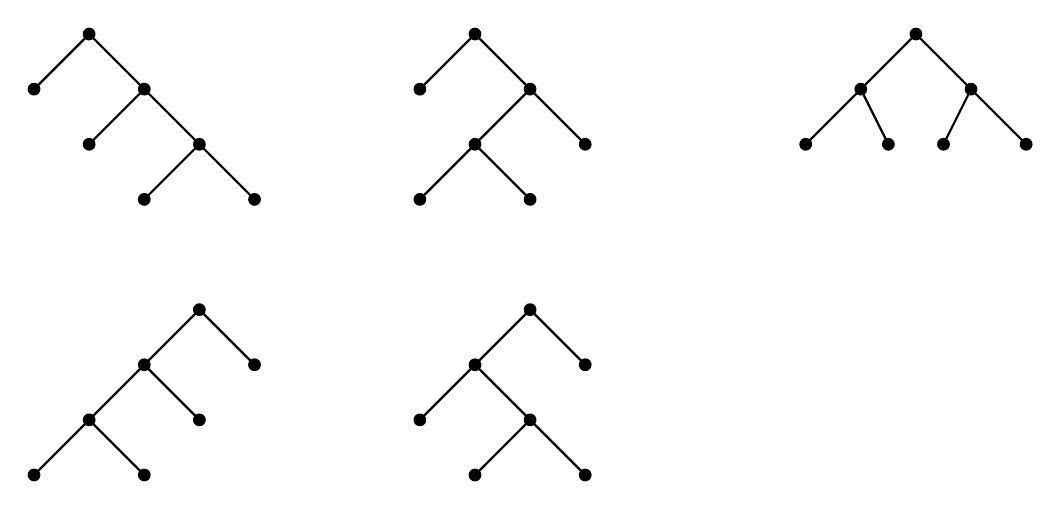
\begin{tikzpicture}[scale = .7]
		\begin{scope}
		\draw[fill] (-1,0) circle (3pt);
		\draw[fill] (0,1) circle (3pt);
		\draw[fill] (0,-1) circle (3pt);
		\draw[fill] (1,0) circle (3pt);
		\draw[fill] (1,-2) circle (3pt);
		\draw[fill] (2,-1) circle (3pt);
		\draw[fill] (3,-2) circle (3pt);
		\draw[thick] (-1,0) -- (0,1) -- (1,0) -- (2,-1) -- (3,-2);
		\draw[thick] (0,-1) -- (1,0);
		\draw[thick] (1,-2) -- (2,-1);
		\draw[fill] (6,0) circle (3pt);
		\draw[fill] (6,-2) circle (3pt);
		\draw[fill] (7,1) circle (3pt);
		\draw[fill] (7,-1) circle (3pt);
		\draw[fill] (8,0) circle (3pt);
		\draw[fill] (8,-2) circle (3pt);
		\draw[fill] (9,-1) circle (3pt);
		\draw[thick] (6,0) -- (7,1) -- (8,0) -- (9,-1);
		\draw[thick] (7,-1) -- (8,0);
		\draw[thick] (6,-2) -- (7,-1) -- (8,-2);
		\draw[fill] (13,-1) circle (3pt);
		\draw[fill] (14,0) circle (3pt);
		\draw[fill] (15,1) circle (3pt);
		\draw[fill] (14.5,-1) circle (3pt);
		\draw[fill] (15.5,-1) circle (3pt);
		\draw[fill] (16,0) circle (3pt);
		\draw[fill] (17,-1) circle (3pt);
		\draw[thick] (13,-1) -- (14,0) -- (15,1) -- (16,0) -- (17,-1);
		\draw[thick] (14.5,-1) -- (14,0);
		\draw[thick] (15.5,-1) -- (16,0);
		\draw[fill] (-1,-7) circle (3pt);
		\draw[fill] (0,-6) circle (3pt);
		\draw[fill] (1,-7) circle (3pt);
		\draw[fill] (1,-5) circle (3pt);
		\draw[fill] (2,-6) circle (3pt);
		\draw[fill] (2,-4) circle (3pt);
		\draw[fill] (3,-5) circle (3pt);
		\draw[thick] (-1,-7) -- (0,-6) -- (1,-5) -- (2,-4) -- (3,-5);
		\draw[thick] (1,-7) -- (0,-6);
		\draw[thick] (2,-6) -- (1,-5);
		\draw[fill] (6,-6) circle (3pt);
		\draw[fill] (7,-7) circle (3pt);
		\draw[fill] (7,-5) circle (3pt);
		\draw[fill] (8,-6) circle (3pt);
		\draw[fill] (8,-4) circle (3pt);
		\draw[fill] (9,-7) circle (3pt);
		\draw[fill] (9,-5) circle (3pt);
		\draw[thick] (6,-6) -- (7,-5) -- (8,-4) -- (9,-5);
		\draw[thick] (7,-5) -- (8,-6) -- (7,-7);
		\draw[thick] (8,-6) -- (9,-7);
		\end{scope}
		
		\end{tikzpicture}
		
	\end{center}
	
	Each binary tree above corresponds to one of the Beveridge sequence with $n = 3$, from left to right: $(1,2,3,3), (1,3,3,2), (2,2,2,2), (3,3,2,1), (2,3,3,1).$
	
	\section{Proof}
	\subsection{Groundwork}
	Let us start by laying down a few theorems and definitions that will be used throughout the rest of the paper. Some theorems will be left unproven as their proof will be left for a real analysis student to complete.
	
	%%% DEFINITION OF SEQUENCE, can be included if desired, however it's a bit much %%%
	%\begin{definition}{Sequence}
	%A sequence is defined as a function $S:[n]\to\mathbb R$. We will write $S_i = S(i)$ for any $i \le n$. Additionally we say that $\cardinality S = n$ and that $i$ is an index in $S$ if $i \in [n]$. We may also define a function by saying $S = (S_1, S_2, S_3, \ldots, S_n)$. An index $i$ is said to come later than $j$ if $i > j$ and thus $j$ would be said to come earlier.
	%\end{definition}
	%%%%%%%%%%%%%%%%%%%%%%%%%%%%%%%%%%%%%%%%%%%%%%%%%%%%%%%%%%%%%%%%%%%%%%%%%%%%%%%%%%%%
	
	\begin{definition}{Beveridge}
		A beveridge sequence is any sequence, $S$, of non-negative integers for which both the following two properties hold.
		\begin{enumerate}
			\item $\sumfrom{i=1}{\cardinality{S}}{2^{-S_i}} = 1$
			\item For all indices $j \in \set{2,3,\ldots,\cardinality{S}}$, $2^{S_j}\sumfrom{i=1}{j-1}{2^{-S_i}}$ is an integer.
		\end{enumerate}
	\end{definition}
	
	\begin{theorem} \label{increasing}
		For any sequence $S$ of real numbers \[\sumfrom{n=1}{k}{2^{-S_n}} > \sumfrom{n=1}{k-1}{2^{-S_n}}\]
		for any integer $k > 1$.
	\end{theorem}
	
	\begin{theorem}	\label{positive}
		If a sequence $S$ is beveridge and $\cardinality{S} > 1$ then all elements in $S$ are positive.
	\end{theorem}
	
	\begin{proof}
		Let $S$ be a beveridge sequence. Thus all elements in $S$ must be non-negative integers. Assume that $S$ contains some index $i$ for which $S_i$ is not positive. Zero is the only non-negative, non-positive integer, thus $S_i = 0$. We know that $2^{-0} = 1$, thus $S$ must only contain $0$ as otherwise \[\sumfrom{n=1}{\cardinality{S}}{2^{-S_n}} > 2^{-S_i} = 1\] which is impossible as $S$ is beveridge. Thus if $S$ contains a non-positive element, then that may be it's only element, making $\cardinality{S} = 1$. If $\cardinality{S} > 1$ then $S$ may only contain non-negative and non-zero integers, which is the same as only containing positive integers.
	\end{proof}
	
	
	\subsection{Midpoint}
	
	
	\begin{theorem}	\label{one}
		If a sequence $S$ is beveridge and $\cardinality{S} > 1$ then there exists exactly one index $p(S)$ such that \[\sumfrom{i=1}{p(S)}{2^{-S_i}} = \frac12\]
	\end{theorem}
	\begin{proof}
		Let $S$ be a beveridge sequence with $\cardinality{S} > 1$. Assume for the sake of contradiction that there does not exist an index $p$ such that $\sumfrom{i=1}{p}{2^{-S_i}} = \frac12$. Because of theorem \ref{increasing}, we know that there is some index, $j$ such that \[\sumfrom{i=1}{j}{2^{-S_i}} > \frac12 > \sumfrom{i=1}{j-1}{2^{-S_i}}\] Because $2^{S_j}$ must be positive regardless of $j$ or $S$, we may multiply it through and our inequality will hold, giving us
		\begin{align*}
			2^{S_j}\sumfrom{i=1}{j}{2^{-S_i}}& \\
			= 1 + &2^{S_j}\sumfrom{i=1}{j-1}{2^{-S_i}}
			> 2^{S_j}\frac12 
			> 2^{S_j}\sumfrom{i=1}{j-1}{2^{-S_i}}
		\end{align*} 
		At this point we must observe that $j > 1$. To prove this we will assume that $j = 1$ (note that $j < 1$ makes no sense as it would be a sum of $0$ things, thus resulting in a result of $0$ which is less then $\frac12$), and we find
		\[
		\sumfrom{i=1}{j}{2^{-S_i}} = \sumfrom{i=1}{1}{2^{-S_i}} = 2^{-S_1} > \frac12
		\]
		and the only non-negative integer value for $S_1$ that satisfies this is $S_1 = 0$, which by theorem \ref{positive} means that $\cardinality{S} = 1$, which is a contradiction as we defined $S$ to have $\cardinality{S} > 1$. We thus know that $j > 1$, and because of that we know that $2^{S_j}\sumfrom{i=1}{j-1}{2^{-S_i}}$ is an integer. Now to finally finish this off we know that for any integer $k$ there are no integers in the interval $\ooint k{k+1}$, thus we know that $2^{S_j}\frac12 = 2^{S_j-1}$ is not an integer. As $S_j$ must be an integer this means that $S_j - 1 < 0$ or alternatively $S_j < 1$ which would mean that $S_j$ is not positive, however by theorem \ref{positive} we know that $S_j$ is positive and thus we have our contradiction.
		
		Finally we notice that there is only one possible point for any beveridge sequence $p$ via theorem \ref{increasing}, any index before $p$ must yield a sum less than $\frac12$ and any index after $p$ must yield a sum greater than $\frac12$.\footnote{When I say sum I really mean a sum in the form $\sumfrom{i=0}{k}{2^{-S_i}}$, where $k$ is some index in $S$.}
		
		Now we have shown that for all beveridge sequences $S$ of length greater than one, there exists a unique index $k$, such that $\sumfrom{i=1}{k}{2^{-S_i}} = \frac12$. Thus we may define a function $p(S) = k$ where \[\sumfrom{i=1}{k}{2^{-S_i}} = \frac12\]
	\end{proof}
	
	
	\begin{theorem}\label{edge}
		For any beveridge sequence $S$ with $\cardinality S > 1$, $p(S) < \cardinality S$.
	\end{theorem}
	
	\begin{proof}
		$S$ is beveridge thus, $\sumfrom{i=1}{\cardinality S}{2^{-S_i}} = 1 > \frac12$, and by theorem    \ref{increasing} we know that $p < \cardinality S$.
	\end{proof}
	
	\subsection{Decomposition}
	
	In this section we will show that using the index $p(S)$ we may break any beveridge sequence $S$ into two smaller beveridge sequences, in exactly one way, as long as $\cardinality S \not= 1$.
	
	\begin{theorem} \label{decompose}
		For any beveridge sequence $S$, of length greater than $1$, there exists two sequences
		\begin{align*}
			L(S) &= (S_1 - 1, S_2 - 1, \ldots, S_{p(S)} - 1) \\
			R(S) &= (S_{p(S)+1} - 1, S_{p(S)+2} - 1, \ldots, S_{\cardinality S} - 1)
		\end{align*}
		both of which are beveridge.
	\end{theorem}
	
	
	\begin{proof}
		Let $S$ be a beveridge sequence with $\cardinality S > 1$. First notice that $\cardinality{L(S)} \ge 1$ and that $\cardinality{R(S)} \ge 1$. $L(S)$ always contains $S_{p(S)}-1$ as an element, thus must contain at least one element. By theorem \ref{edge} we know that $p(S) + 1 < \cardinality S$, thus $S_{p(s)+1}-1$ is always in $R(S)$, so $R(S)$ may also not be empty. Second we would also like to notice that $L(S)$ and $R(S)$ contain only non-negative integers, as $S$ contains only positive integers (see theorem \ref{positive}).
		
		Now that we have shown that $L(S)$ and $R(S)$ are non-empty sequences of non-negative integers, we can start to show that they fit the requirements to be beveridge, this is simply a fair amount of fairly simple manipulation.
		
		First we want to show that $\sumfrom{i=1}{\cardinality{L(S)}}{2^{-L(S)_i}} = 1$.
		\begin{align*}
			\sumfrom{i=1}{\cardinality{L(S)}}{2^{-L(S)_i}} 
			&= \sumfrom{i=1}{p}{2^{-(S_i-1)}}\\
			&= \sumfrom{i=1}{p}{2^{-S_i+1}} \\
			&= 2\sumfrom{i=1}{p}{2^{-S_i}}
			= 2\cdot\frac12
			= 1
		\end{align*}
		
		Next we wish to show that $\sumfrom{i=1}{\cardinality{R(S)}}{2^{-R(S)_i}} = 1$.
		\begin{align*}
			\sumfrom{i=1}{\cardinality{R(S)}}{2^{-R(S)_i}}
			&= \sumfrom{i=p+1}{\cardinality{S}}{2^{-(S_i-1)}} \\
			&= \sumfrom{i=p+1}{\cardinality S}{2^{-S_i+1}} \\
			&= 2\sumfrom{i=p+1}{\cardinality S}{2^{-S_i}} \\
			&= 2\left[\sumfrom{i=1}{\cardinality S}{2^{-S_i}} - \sumfrom{i=1}{p}{2^{-S_i}}\right]
			= 2\left[1-\frac12\right]
			= 1
		\end{align*}
		
		Next we will show that for any $j \in \set{2, 3, \ldots, \cardinality{L(S)}}$, $\sumfrom{i=1}{j-1}{2^{L(S)_j-L(S)_i}}$ is an integer. Let us start by choosing $j \in \set{2, 3, \ldots, \cardinality{L(S)}}$.
		\begin{align*}
			\sumfrom{i=1}{j-1}{2^{L(S)_j - L(S)_i}}
			&= \sumfrom{i=1}{j-1}{2^{(S_j - 1) - (S_i - 1)}} \\
			&= \sumfrom{i=1}{j-1}{2^{S_j - S_i}} \in \mathbb Z
		\end{align*}
		We know this is an integer as $S$ is beveridge, thus we have shown that $L(S)$ is beveridge.
		
		Finally we will show that for any $j \in \set{2, 3, \ldots, \cardinality{R(S)}}$, $\sumfrom{i=1}{j-1}{2^{R(S)_j-R(S)_i}}$ is an integer.
		\begin{align*}
			\sumfrom{i=1}{j-1}{2^{R(S)_j-R(S)_i}}
			&= \sumfrom{i=p+1}{j-1 + p}{2^{(S_j - 1) - (S_i - 1)}} \\
			&= \sumfrom{i=p + 1}{j-1 + p}{2^{S_j - S_i}}\\
			&= \sumfrom{i=1}{j-1+p}{2^{S_j-S_i}} - \sumfrom{i=1}{p}{2^{S_j-S_i}}\\
			&= \sumfrom{i=1}{j-1+p}{2^{S_j - S_i}} - 2^{S_j}\cdot\frac12
		\end{align*}
		Now we notice that $\sumfrom{i=1}{j-1+p}{2^{S_j-S_i}}$ is an integer as $S$ is beveridge and $j\not= 1$. Additionally we know that $S_j$ is positive via theorem \ref{positive} and thus $S_j-1 \ge 0$. Also notice that $2^{S_j}\cdot\frac12 = 2^{S_j - 1}$, and as $S_j-1$ is non-negative, $2^{S_j-1}$ must be an integer. Finally the integers are closed on addition so we know $\sumfrom{i=1}{j-1+p}{2^{S_j - S_i}} - 2^{S_j}\cdot\frac12$ is an integer. Now we have shown that $R(S)$ is beveridge.
	\end{proof}
	
	%Consider the Beveridge Sequence $a_1, a_2, \ldots , a_{n}$, where $n > 1$. Theorem \ref{one} has it that there exists some index $k$, for whichdd
	%\[dd
	%\sum_{i=1}^k 2^{-a_i} = \frac{1}{2}.dd
	%\]dd
	%We will prove that this index breaks the sequence into two subsequences such that if we subtract one from every element of each subsequence, we get a valid Beveridge Sequence. Let the sequence $L = (a_1 - 1, a_2 - 2, \ldots, a_p - 1)$ and the sequence $R = (a_{p+1} - 1, a_{p+2} - 1, \ldots, a_{n} - 1)$. Now we wish to show that both $L$ and $R$ are beveridge.dd
	%dd
	%\begin{enumerate}dd
	%\item[(1)] First, we need to prove thatdd
	%\[dd
	%\sum_{i=1}^k 2^{-(a_i-1)} = 1dd
	%\]dd
	%anddd
	%\[dd
	%\forall j: 2 \leq j \leq k, \text{ we have } 2^{a_j-1} \sum_{i=1}^{j-1} 2^{-(a_i-1)} \in \mathbb{Z}.dd
	%\]dd
	%dd
	%\begin{itemize}dd
	%\item We have:dd
	%\begin{align*}dd
	%\sum_{i=1}^k 2^{-(a_i-1)} &= \sum_{i=1}^k \frac{1}{2^{a_i -1}} \\dd
	%&= \sum_{i=1}^k \frac{1}{2^{a_i}\cdot 2^{-1}} \\dd
	%&= \sum_{i=1}^k \frac{1}{2^{a_i}} \cdot 2 \\dd
	%&= \sum_{i=1}^k 2^{-a_i} \cdot 2  \\dd
	%&= \frac{1}{2} \cdot 2 = 1.dd
	%\end{align*}dd
	%\item Now we prove the second part, i.e. for all $j$, where $2\leq j \leq k+1$ such that dd
	%\[dd
	%2^{a_j} \sum_{i=1}^{j-1} 2^{-(a_i-1)} \in \mathbb{Z}.dd
	%\]dd
	%dd
	%We have:dd
	%\begin{align*}dd
	%2^{a_j-1} \sum_{i=1}^{j-1} 2^{-(a_i-1)} &= \frac{2^{a_j}}{2} \sum_{i=1}^{j-1} \frac{1}{2^{a_i -1}} \\dd
	%&= \frac{2^{a_j}}{2} \sum_{i=1}^{j-1}\frac{1}{2^{a_i}} \cdot 2 \\dd
	%& = 2^{a_j} \sum_{i=1}^{j-1} \frac{1}{2^{a_i}}.dd
	%\end{align*}dd
	%The second property of the Beveridge Sequence has it that this value is an integer.dd
	%\end{itemize}dd
	%dd
	%Thus, we have proved that the part on the left of the "dividing" index $k$ is a valid Beveridge Sequence.dd
	%dd
	%\item[(2)] Similarly, we can prove that the part on the right of the "dividing" index $k$ is also a valid Beveridge Sequence. In order to do that, we will prove that dd
	%\[dd
	%\sum_{i=k+1}^{n+1} 2^{-(a_i-1)} = 1dd
	%\]dd
	%and dd
	%\[dd
	%\forall j: k+2 \leq j \leq n+1, \text{ we have } 2^{a_j-1} \sum_{i=1}^{j-1} 2^{-(a_i-1)} \in \mathbb{Z}.dd
	%\]dd
	%dd
	%\begin{itemize}dd
	%\item We have:dd
	%\begin{align*}dd
	%\sum_{i=k+1}^{n+1} 2^{-(a_i-1)} &= \sum_{i=k+1}^{n+1} \frac{1}{2^{a_i}} \frac{1}{2^{-1}} \\dd
	%&= \sum_{i=k+1}^{n+1} \frac{1}{2^{a_i}} \cdot 2 \\dd
	%&= \frac{1}{2} \cdot 2 = 1.dd
	%\end{align*}dd
	%dd
	%\item We now prove the second part, i.e. for all $j$, where $2 \leq j \leq k+1$ such that dd
	%\[dd
	%2^{a_j-1} \sum_{i=1}^{j-1} 2^{-(a_i-1)} \in \mathbb{Z}.dd
	%\]dd
	%dd
	%We have:dd
	%\begin{align*}dd
	%2^{a_j-1} \sum_{i=1}^{j-1} 2^{-(a_i-1)} &= \sum_{i=1}^{j-1} 2^{a_j-a_i} \\dd
	%&= \sum_{i=k+1}^{k+j-1} 2^{a_j-a_i} \\dd
	%&= 2^{a_j} \sum_{i=1}^{k+j-1} 2^{-a_i} - 2^{a_j}\sum_{i=1}^k \\dd
	%&= 2^{a_j} \sum_{i=1}^{k+i-1} - 2^{a_j-1} \in \mathbb{Z}.dd
	%\end{align*}dd
	%\end{itemize}dd
	%\end{enumerate}dd
	%Thus, we have proved that the index $k$ divides the sequence into two subsequences that satisfy the conditions.
	
	\subsection{Composition}
	In the last section we showed that one could decompose any beveridge sequence $S$ of length greater than $1$ into two smaller beveridge sequences. We now want to show that if we take two beveridge sequences $L$ and $R$ we can compose them to construct a larger beveridge sequence. Let us start by defining a composition function \[C(L,R) = (L_1 + 1, L_2 + 1, \ldots, L_{\cardinality L} + 1,\quad R_1 + 1, R_2 + 1, \ldots, R_{\cardinality R} + 1)\]
	
	
	\begin{theorem} \label{compose}
		If $L$ and $R$ and beveridge sequences then $C(L,R)$ is also beveridge.
	\end{theorem}
	
	\begin{proof}
		Let $L$ and $R$ be beveridge sequences. First let us notice that $C(L,R)$ is a sequence of positive integers, as $L$ and $R$ are both sequences of non-negative integers.
		
		Next we would like to show that $\sumfrom{i=1}{\cardinality{C(L,R)}}{2^{-C(L,R)_i}}=1$.
		\begin{align*}
			\sumfrom{i=1}{\cardinality{C(L,R)}}{2^{-C(L,R)_i}}
			&= \sumfrom{i=1}{\cardinality{L}}{2^{-(L_i + 1)}} + \sumfrom{i=1}{\cardinality{R}}{2^{-(R_i+1)}} \\
			&= \frac12\left[\sumfrom{i=1}{\cardinality L}{2^{-L_i}} + \sumfrom{i=1}{\cardinality{R}}{2^{-R_i}}\right] \\
			&= \frac12\left[1 + 1\right]
			= 1
		\end{align*}
		
		Finally we would like to show that for any $j \in \set{2, 3, \ldots, \cardinality{C(L,R)}}$, $\sumfrom{i=1}{j-1}{2^{C(L,R)_j-C(L,R)_i}}$ is an integer. To do this we must do a proof by cases. Let us consider the three possible cases:
		\begin{enumerate}
			\item$j < \cardinality L + 1$
			\item$j = \cardinality L + 1$
			\item$j > \cardinality L + 1$
		\end{enumerate}
		
		First if $j < \cardinality L + 1$, this is the same as saying $j \in \set{2, 3, \ldots, \cardinality L}$.
		First we should notice that
		\[
		\sumfrom{i=1}{j-1}{2^{C(L,R)_j-C(L,R)_i}} = \sumfrom{i=1}{j-1}{2^{(L_j+1)-(L_i+1)}}
		\]
		as we are never referencing any index in $C(L,R)$ after the $j^\text{th}$ index which we know is at most $\cardinality L$. Now we simplify and find
		\[
		\sumfrom{i=1}{j-1}{2^{(L_j+1)-(L_i+1)}} = \sumfrom{i=1}{j-1}{2^{L_j-L_i}} \in \mathbb Z
		\]
		as $L$ is beveridge.
		
		Second if $j = \cardinality L + 1$, this means that we want to show that $\sumfrom{i=1}{\cardinality L}{2^{C(L,R)_{\cardinality L}-C(L,R)_i}}$ is an integer. Let us start by rewriting this as $2^{C(L,R)_{\cardinality L + 1}}\sumfrom{i=1}{\cardinality L}{2^{-C(L,R)_i}}$. Now we notice that $\sumfrom{i=1}{\cardinality L}{2^{-C(L,R)_i}} = \sumfrom{i=1}{\cardinality L}{2^{-(L_i + 1)}}$. Well we now show that
		\[\sumfrom{i=1}{\cardinality L}{2^{-(L_i + 1)}} = \frac12\sumfrom{i=1}{\cardinality L}{2^{-L_i}} = \frac12\cdot 1 = \frac12\]
		We now look at the $2^{C(L,R)_{\cardinality L + 1}}$ part. Notice that $C(L,R)_{\cardinality L + 1} = R_1 + 1$, thus $2^{C(L,R)_{\cardinality L + 1}} = 2^{R_1 + 1}$. Now we may put the parts together and we find that
		\[\sumfrom{i=1}{\cardinality L}{2^{C(L,R)_{\cardinality L}-C(L,R)_i}} = 2^{R_1 + 1}\cdot\frac12 - 2^{R_1}\]
		which is an integer as $R$ is composed of non-negative integers.
		
		Finally if $j > \cardinality L + 1$ we may do the following manipulation.
		\begin{align*}
			\sumfrom{i=1}{j-1}{2^{C(L,R)_j-C(L,R)_i}}
			&= 2^{C(L,R)_j}\sumfrom{i=1}{j-1}{2^{-C(L,R)_i}} \\
			&= 2^{R_{j-\cardinality L}+1}\left[ \sumfrom{i=1}{\cardinality L}{2^{-(L_i + 1)}} + \sumfrom{i=1}{j-1-\cardinality{L}}{2^{-(R_i + 1)}} \right] \\
			&= 2^{R_{j-\cardinality L} + 1}\cdot\frac12\left[1 +  \sumfrom{i=1}{j-1-\cardinality{L}}{2^{-R_i}}\right] \\
			&= 2^{R_{j-\cardinality L}} + 2^{R_{j-\cardinality L}}\sumfrom{i=1}{j-\cardinality{L}-1}{2^{-R_i}}
		\end{align*}
		Now $j-\cardinality L$ must be a member of $\set{2,3,\ldots,\cardinality R}$ and so we know that $2^{R_{j-\cardinality L}}\sumfrom{i=1}{j-\cardinality{L}-1}{2^{-R_i}}$ is an integer as $R$ is beveridge, thus we have the sum of two integers, and that must be an integer.
		
		Now we have demonstrated that for any pair of beveridge sequences $L$ and $R$, $C(L,R)$ is beveridge.
	\end{proof}
	
	We now must demonstrate that if we have two separate pairs of beveridge sequences we can't possibly compose both pairs respectively and get the same sequence
	
	\begin{theorem} \label{unique}
		If $A$, $B$, $\bar A$ and $\bar B$ are beveridge sequences such that $A \not= \bar A$ or $B \not= \bar B$  then $C(A,B) \not= C(\bar A, \bar B)$.
	\end{theorem}
	\begin{proof}
		This will be a proof by contra-positive. First we state
		\[\sumfrom{i=1}{\cardinality L}{2^{-C(L,R)_i}} = \sumfrom{i=1}{\cardinality L}{2^{-L_i - 1}} = \sumfrom{i=1}{\cardinality L}{2^{-L_i}}\cdot \frac 12 = \frac12\]
		and we find that the sum across the first $\cardinality L$ terms of $2^{-C(L,R)}$ is $\frac12$, thus $L = L(C(L,R))$, and thus there is exactly one way to construct $L$ from $C(L,R)$ and further there will be exactly one way to construct $R$. Thus we know that compositions are unique.
	\end{proof}
	
	\section{Complete induction}
	Here we will finally prove that there are $C_n$ beveridge sequences of length $n+1$, where $C_n$ is the $n^\text{th}$ Catalan number defined as \begin{align*}C_0& = 1 \\ C_n& = \sum_{i=0}^{n-1}C_i\cdot C_{n-i-1}\end{align*}
	
	\begin{proof}
		First we wish to show that there is exactly one beveridge sequence of length $1$. If a sequence is beveridge and of length one then we know that $\sumfrom{i=1}1{2^{-A_i}} = 1$, where $A$ is our beveridge sequence. We may rewrite this without the sigma as $2^{-A_1} = 1$. There is only one possible non-negative integer value for $A_1$, and this is $0$. Thus the sequence $(0)$ is the only sequence of length $1$ that is beveridge.\footnote{Technically I haven't shown that $(0)$ is beveridge, however it is rather trivial.} Now we have shown a base case
		
		Now choose $k \in \mathbb N$, let us assume that for all non-negative integers $n < k$, the number of beveridge sequences of length $n + 1$ is $C_n$. Now we wish to show that there are exactly $C_{k}$ beveridge sequences of length $k + 1$. First by theorem \ref{decompose} we know that all beveridge sequences of length $k+ 1$ can be decomposed into two shorter beveridge sequences. Next by theorem \ref{compose} and \ref{unique} we know that each composition of two beveridge sequences produces a unique beveridge sequence with length $l+r$ where $l$ and $r$ are the lengths of the two sequences being composed respectively. Thus for every beveridge sequence of length $t<k + 1$ (of which there are $C_{t-1}$) we may compose it with a beveridge sequence of length $k + 1 - t$ (of which there are $C_{k-t}$) to get a unique beveridge sequence of length $k + 1$. Thus we find that there are $\sumfrom{t=1}{k}{C_{t-1}\cdot C_{k-t}} = \sumfrom{i=0}{k-1}{C_{i}\cdot C_{k-i-1}}$ beveridge sequences of length $k + 1$ that can be composed of smaller beveridge sequences, this is of course all of them as we have already stated.
		
		Now by the principle of complete induction we know there are $C_n$ beveridge sequences of length $n + 1$.
	\end{proof}
	
	
	
	%\section{Weak Induction}
	%Assume that the there are $c_n$ beveridge sequences of length $n+1$.  That being said $c_0=1$ because there are only one sequence of length 1, $0$.  Now we prove that there are $c_{k-1}$ sequences of length $k$.  We can split these sequences, of length $k$, into two sub-sequences that are still sequences (proof from above).  We define these sub-sequences as 
	%$$
	%a_1, \ldots, a_j\quad a_{j+1}, \ldots, a_k$$
	%where the lengths of the subsections are $j$ and $k-j$ respectively, where $1\le j \le k$.  Using our assumption about beveridge sequences, there are $c_{j-1}$ sequences of length $j$ and $c_{k-j-1}$ of length $n-j$ where $1\le j \le k$.  The total number of possible sequences for length $k$ are $c_{j-1}\cdot c_{k-j-1}$ where $1\le j \le k-1$.
	%
	%\begin{eqnarray*}
	%\sum_{j=1}^{k-1} c_j \cdot c_{k-j-1} \\
	%\sum_{i=0}^{k-2} c_i \cdot c_{k-i-2}
	%\end{eqnarray*}
	%Notice that the summation is very similar to the Catalan recurrence:
	%\begin{eqnarray*}
	%C_0 &=& 1 \\
	%C_{n+1} &=& \sum_{i=0}^n C_i C_{n-i-1} \mbox{ for } n \geq 0.
	%\end{eqnarray*}
	%Therefore there are $c_{k-1}$ beveridge sequences for length $k$.
	%
	%
	
	
	
\end{document}
